\documentclass[11pt]{article}
\usepackage{tikz}
\usetikzlibrary{trees}
\usepackage{forest}
\usepackage{hyperref}
\usepackage{multirow}
\usepackage{graphicx}


%Gummi|065|=)
\title{\textbf{Shannon Entropy}}
\author{K{\i}van\c{c} \c{C}akmak\\}
\date{}
\begin{document}

\maketitle

In this article, I'll try to explain Shannon Entropy with one of it's use case: data-compression. First, I'll provide a small introduction about data-representation and a need for compression with a very brief information about it's requirements. Consequently, I'll derive the proof of well known entropy formula in the equation below:

\begin{equation}
H(X) = -\sum_{i}p_{i}\log_{b}p_{i}
\label{Eq:entropy}
\end{equation}

\section{Data Representation and Compression}

We all know that the way that our digital devices store data is ones and zeros, aka in binary format. So, our understanding of the smallest chunk of information is: "whether there is a voltage or not". 
We represent letters of a text, pixels of an image, etc. in binary format. 

Below, I provide an ASCII (American Standard Code for Information Interchange) encoded \textit{hello} in Table \ref{table:hello}. In ASCII, each letter -and other control characters, such as \texttt{DEL} and numbers like $1$, $2$ etc.- consists $8$ bits. So, the text that we see is \texttt{hello}, but the information that a digital device store is: 
\begin{center}
    \texttt{0110100001100101011011000110110001101111}
\end{center}

\begin{figure}
\begin{tabular}{| l | l | l | l | l | l |}
 \hline
  text   & h & e & l & l & o\\ \hline
  ASCII  & 104 & 101 & 108 & 108 & 111 \\ \hline 
  binary & 01101000 & 01100101 & 01101100 & 01101100 & 01101111 \\ 
  \hline
\end{tabular}
\caption{ASCII encoding of \textit{hello}.}
\label{table:hello}
\end{figure}

So, there are $26$ letters in the English alphabet, and we can say that $5$ bits would be enough to encode all characters, since $2^{5} = 32 > 26$. Nevertheless, ASCII has 127 different values --See Reference \cite{ascii}, which at least requires 7 bits per value. 

\newpage
The rest of the document tries to answer the following question:

\begin{center}
\textit{What would be the minimum number of bits that we have to use, if we knew the distribution of letters in the text?}
\end{center}

\begin{figure}[ht!]
\centering
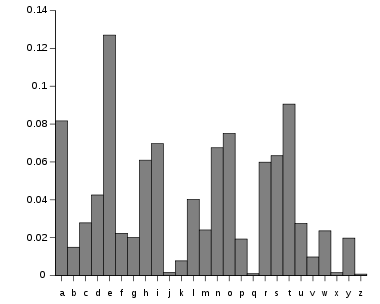
\includegraphics[width=\linewidth]{img/english_histogram.png}
\caption{Frequency Table of English Letters \label{fig:letter_histogram}}
\end{figure}

So, as it could be seen in the Figure \ref{fig:letter_histogram} --and we all very well know, some of the letters are more oftenly used than the others. Here, \textit{e} is the most commonly used letter in English. So, would it be better to represent \textit{e} with less bits than the others, if the letter distribution of our text would be exactly same with Figure \ref{fig:letter_histogram}. If so, how less should it be?

\section{Uniquely Decodable Codes}
TODO: uniquely decodable codes.

\subsection{Prefix Codes}
TODO: prefix codes.

\section{Kraft's Inequality}

\begin{center}
\begin{forest}
for tree={circle,draw, l sep=1cm, s sep=1.5cm, minimum height=0.8cm, minimum width=1cm}
[, 
    [0,edge label={node[midway,left] {$2^{-1}$}}]
    [,edge label={node[midway,right] {$2^{-1}$}}
      [10,edge label={node[midway,left] {$2^{-2}$}}] 
      [,edge label={node[midway,right] {$2^{-2}$}}
      [110,edge label={node[midway,left] {$2^{-3}$}}]
      [111,edge label={node[midway,right] {$2^{-3}$}}]
      ] 
  ] 
]
\end{forest}
\end{center}


\begin{thebibliography}{99}


\bibitem{ascii}
\url{http://ee.hawaii.edu/~tep/EE160/Book/chap4/subsection2.1.1.1.html}

\bibitem{mortada_krafts}
\url{https://mortada.net/simple-proof-for-krafts-inequality.html}


\end{thebibliography}


\end{document}
